% Practice Test 25 — Texas Edition
% Questions: 30 (21 MC + 9 SA)
% Generated by scripts/generate_practice_tests.py

\begin{practiceQuestion}{1-3-q26}{gmc}
\begin{questionText}
The graph below shows a proportional relationship. What is the constant of proportionality?

\begin{center}
\begin{tikzpicture}[scale=0.8]
  \draw[step=1,gray!20,thin] (0,0) grid (6,6);
  \draw[thick,->] (0,0) -- (6.5,0) node[right]{\small $x$};
  \draw[thick,->] (0,0) -- (0,6.5) node[above]{\small $y$};
  \foreach \x in {1,...,6} \draw (\x,0.07) -- (\x,-0.07) node[below]{\tiny \x};
  \foreach \y in {1,...,6} \draw (0.07,\y) -- (-0.07,\y) node[left]{\tiny \y};
  \draw[thick,funBlue] (0,0) -- (6,4);
  \fill[funBlue] (0,0) circle (2.5pt);
  \fill[funBlue] (3,2) circle (2.5pt) node[above left]{\small $(3, 2)$};
  \fill[funBlue] (6,4) circle (2.5pt) node[above left]{\small $(6, 4)$};
\end{tikzpicture}
\end{center}
\end{questionText}
\choiceA{$k = \frac{1}{2}$}
\choiceB{$k = \frac{2}{3}$}
\choiceC{$k = \frac{3}{2}$}
\choiceD{$k = 2$}
\correctAnswer{B}
\explanation{Use any labeled point: $k = \frac{2}{3}$ from $(3, 2)$. Check: $\frac{4}{6} = \frac{2}{3}$ \checkmark.}
\end{practiceQuestion}

\begin{practiceQuestion}{1-6-q26}{gmc}
\begin{questionText}
The table shows the distance a bus travels over several hours. Using proportional reasoning, how far will the bus travel in $9$ hours?

\begin{center}
\begin{tabular}{|c|c|}
\hline
\textbf{Hours} & \textbf{Miles} \\ \hline
$2$ & $90$ \\ \hline
$5$ & $225$ \\ \hline
$7$ & $315$ \\ \hline
$9$ & $?$ \\ \hline
\end{tabular}
\end{center}
\end{questionText}
\choiceA{$360$ miles}
\choiceB{$385$ miles}
\choiceC{$405$ miles}
\choiceD{$450$ miles}
\correctAnswer{C}
\explanation{Rate: $90 \div 2 = 45$ mph. In $9$ hours: $45 \times 9 = 405$ miles.}
\end{practiceQuestion}

\begin{practiceQuestion}{2-1-q02}{mc}
\begin{questionText}
$18$ is what percent of $72$?
\end{questionText}
\choiceA{$18\%$}
\choiceB{$20\%$}
\choiceC{$25\%$}
\choiceD{$36\%$}
\correctAnswer{C}
\explanation{Divide the part by the whole: $18 \div 72 = 0.25 = 25\%$.}
\end{practiceQuestion}

\begin{practiceQuestion}{2-3-q15}{mc}
\begin{questionText}
Which of the following results in the greatest final value, starting from $\$100$?
\end{questionText}
\choiceA{Increase by $30\%$}
\choiceB{Increase by $20\%$, then increase by $10\%$}
\choiceC{Increase by $15\%$ twice}
\choiceD{All give the same result}
\correctAnswer{C}
\explanation{A: $100 \times 1.30 = 130$. B: $100 \times 1.20 \times 1.10 = 132$. C: $100 \times 1.15 \times 1.15 = 132.25$. C is the greatest.}
\end{practiceQuestion}

\begin{practiceQuestion}{2-6-q18}{mc}
\begin{questionText}
A $\$1{,}600$ loan at $5.5\%$ simple interest accrues $\$264$ interest. How long was the loan?
\end{questionText}
\choiceA{$2$ years}
\choiceB{$3$ years}
\choiceC{$4$ years}
\choiceD{$5$ years}
\correctAnswer{B}
\explanation{$264 = 1{,}600 \times 0.055 \times t$ → $264 = 88t$ → $t = 3$ years.}
\end{practiceQuestion}

\begin{practiceQuestion}{2-8-q30}{gsa}
\begin{questionText}
The bar graph shows the annual fees at two banks and the annual interest earned on a $\$2{,}000$ deposit. Which bank is the better deal, and how much more do you gain (or save) per year by choosing it?

\begin{center}
\begin{tikzpicture}[scale=0.6]
  \draw[thick,->] (0,0) -- (0,6) node[above] {\$};
  \draw[thick,->] (0,0) -- (10,0);
  \foreach \y/\label in {0/0, 1/10, 2/20, 3/30, 4/40, 5/50} {
    \draw (-0.1,\y) -- (0.1,\y);
    \node[left] at (-0.15,\y) {\footnotesize \$\label};
  }
  % Bank P - Fee
  \fill[funRed!60] (0.5,0) rectangle (1.8,3.6);
  \node[below] at (1.15,-0.1) {\footnotesize Fee};
  \node[above] at (1.15,3.6) {\footnotesize \$36};
  % Bank P - Interest
  \fill[funBlue!60] (2.2,0) rectangle (3.5,4);
  \node[below] at (2.85,-0.1) {\footnotesize Interest};
  \node[above] at (2.85,4) {\footnotesize \$40};
  \node[below] at (2,-.8) {\footnotesize Bank P};

  % Bank Q - Fee
  \fill[funRed!60] (5.5,0) rectangle (6.8,1.2);
  \node[below] at (6.15,-0.1) {\footnotesize Fee};
  \node[above] at (6.15,1.2) {\footnotesize \$12};
  % Bank Q - Interest
  \fill[funBlue!60] (7.2,0) rectangle (8.5,3);
  \node[below] at (7.85,-0.1) {\footnotesize Interest};
  \node[above] at (7.85,3) {\footnotesize \$30};
  \node[below] at (7,-.8) {\footnotesize Bank Q};
\end{tikzpicture}
\end{center}
\end{questionText}
\correctAnswer{Bank Q by $\$14$}
\explanation{Bank P net: $40 - 36 = \$4$ gain. Bank Q net: $30 - 12 = \$18$ gain. Bank Q is better by $18 - 4 = \$14$.}
\end{practiceQuestion}

\begin{practiceQuestion}{2-9-q20}{sa}
\begin{questionText}
You want to save $\$1{,}800$ in $12$ months. How much must you save per month?
\end{questionText}
\correctAnswer{$\$150$}
\explanation{$1{,}800 \div 12 = \$150$ per month.}
\end{practiceQuestion}

\begin{practiceQuestion}{2-10-q22}{sa}
\begin{questionText}
How much more does compound interest earn than simple interest on $\$500$ at $8\%$ for $3$ years?
\end{questionText}
\correctAnswer{$\$9.86$}
\explanation{Simple: $I = 500 \times 0.08 \times 3 = \$120$, total $= \$620$. Compound: $A = 500(1.08)^3 = 500 \times 1.259712 = \$629.86$. Difference: $629.86 - 620 = \$9.86$.}
\end{practiceQuestion}

\begin{practiceQuestion}{4-1-q04}{mc}
\begin{questionText}
Evaluate $2a + 7$ when $a = -3$.
\end{questionText}
\choiceA{$13$}
\choiceB{$1$}
\choiceC{$-13$}
\choiceD{$-1$}
\correctAnswer{B}
\explanation{Substitute: $2(-3) + 7 = -6 + 7 = 1$.}
\end{practiceQuestion}

\begin{practiceQuestion}{4-2-q04}{mc}
\begin{questionText}
Simplify $3y + 8 - 5y - 2$.
\end{questionText}
\choiceA{$8y + 6$}
\choiceB{$-2y + 6$}
\choiceC{$2y - 6$}
\choiceD{$-2y + 10$}
\correctAnswer{B}
\explanation{Combine variable terms: $3y - 5y = -2y$. Combine constants: $8 - 2 = 6$. Result: $-2y + 6$.}
\end{practiceQuestion}

\begin{practiceQuestion}{5-3-q29}{gsa}
\begin{questionText}
The total area of the figure below is $84$ square cm. Find $x$.

\begin{center}
\begin{tikzpicture}[scale=0.5]
  % 6 identical rectangles side by side
  \foreach \i in {0,...,5} {
    \draw[thick,fill=funBlue!15] (\i*2,0) rectangle (\i*2+2,3);
  }
  \draw[<->] (0,-0.7) -- (12,-0.7);
  \node[below] at (6,-0.7) {$6$ rectangles, each width $(x + 1)$ cm};
  \draw[<->] (-0.7,0) -- (-0.7,3);
  \node[left] at (-0.7,1.5) {$2$ cm};
  \node at (6,4.2) {Total area $= 84$ sq. cm};
\end{tikzpicture}
\end{center}
\end{questionText}
\correctAnswer{$x = 6$}
\explanation{Total area $= 6 \times 2 \times (x + 1) = 84$. So $12(x + 1) = 84$. Divide by $12$: $x + 1 = 7$. Subtract $1$: $x = 6$.}
\end{practiceQuestion}

\begin{practiceQuestion}{5-4-q14}{mc}
\begin{questionText}
Solve $0.6x - 2.4 = 1.2$.
\end{questionText}
\choiceA{$x = 6$}
\choiceB{$x = -2$}
\choiceC{$x = 2$}
\choiceD{$x = 0.6$}
\correctAnswer{A}
\explanation{Add $2.4$: $0.6x = 3.6$. Divide by $0.6$: $x = 6$. Check: $0.6(6) - 2.4 = 3.6 - 2.4 = 1.2$ \checkmark.}
\end{practiceQuestion}

\begin{practiceQuestion}{5-5-q29}{gsa}
\begin{questionText}
The balance scale tips to the left. Write and solve the inequality that describes this situation.

\begin{center}
\begin{tikzpicture}[scale=0.7]
  % Tilted beam (left side heavier)
  \draw[thick] (0,-0.5) -- (-0.4,-1.2) -- (0.4,-1.2) -- cycle;
  \draw[thick] (-4.5,0.5) -- (4.5,-0.5);
  % Left pan (lower = heavier)
  \draw[thick] (-4.5,0.5) -- (-5.3,0) -- (-3.7,0) -- (-4.5,0.5);
  \draw[thick,fill=funBlue!20] (-5.3,0) -- (-5.3,-0.4) -- (-3.7,-0.4) -- (-3.7,0) -- cycle;
  \node at (-4.5,-0.2) {$2x + 8$};
  % Right pan (higher = lighter)
  \draw[thick] (4.5,-0.5) -- (5.3,-1) -- (3.7,-1) -- (4.5,-0.5);
  \draw[thick,fill=funOrange!20] (3.7,-1) -- (3.7,-1.4) -- (5.3,-1.4) -- (5.3,-1) -- cycle;
  \node at (4.5,-1.2) {$20$};
\end{tikzpicture}
\end{center}
\end{questionText}
\correctAnswer{$2x + 8 > 20$; $x > 6$}
\explanation{The left side is heavier (tips down), so $2x + 8 > 20$. Subtract $8$: $2x > 12$. Divide by $2$: $x > 6$.}
\end{practiceQuestion}

\begin{practiceQuestion}{5-6-q18}{mc}
\begin{questionText}
Solve $6 - 2x \leq -4$ and describe the graph.
\end{questionText}
\choiceA{Closed circle at $5$, shade right}
\choiceB{Open circle at $5$, shade right}
\choiceC{Closed circle at $5$, shade left}
\choiceD{Closed circle at $-5$, shade right}
\correctAnswer{A}
\explanation{Subtract $6$: $-2x \leq -10$. Divide by $-2$ and flip: $x \geq 5$. Closed circle at $5$, shade right.}
\end{practiceQuestion}

\begin{practiceQuestion}{6-2-q18}{mc}
\begin{questionText}
A drawing uses $1$ cm $= 5$ km. A road is $7$ cm long. Another map shows the same road as $3.5$ cm. What is the scale of the second map?
\end{questionText}
\choiceA{$1$ cm $= 2.5$ km}
\choiceB{$1$ cm $= 5$ km}
\choiceC{$1$ cm $= 10$ km}
\choiceD{$1$ cm $= 17.5$ km}
\correctAnswer{C}
\explanation{Actual road: $7 \times 5 = 35$ km. New scale: $35 \div 3.5 = 10$. So the second map uses $1$ cm $= 10$ km.}
\end{practiceQuestion}

\begin{practiceQuestion}{6-3-q19}{sa}
\begin{questionText}
Can a triangle have sides $10$ cm, $6$ cm, and $3$ cm? Explain why or why not.
\end{questionText}
\correctAnswer{No}
\explanation{$6 + 3 = 9 < 10$. The two shorter sides cannot span the longest side. The triangle inequality is not satisfied.}
\end{practiceQuestion}

\begin{practiceQuestion}{6-4-q13}{mc}
\begin{questionText}
Can a triangle have angles $90°$, $100°$, and $-10°$?
\end{questionText}
\choiceA{Yes, it is a right triangle}
\choiceB{Yes, because the sum is $180°$}
\choiceC{No, because an angle cannot be negative}
\choiceD{No, because the sum is not $180°$}
\correctAnswer{C}
\explanation{Although $90 + 100 + (-10) = 180$, every angle in a triangle must be greater than $0°$. A negative angle is impossible.}
\end{practiceQuestion}

\begin{practiceQuestion}{6-5-q29}{gsa}
\begin{questionText}
The diagram shows a cylinder with radius $4$ cm and height $9$ cm. A vertical cut is made through the center. Describe the cross-section and give its dimensions.

\begin{center}
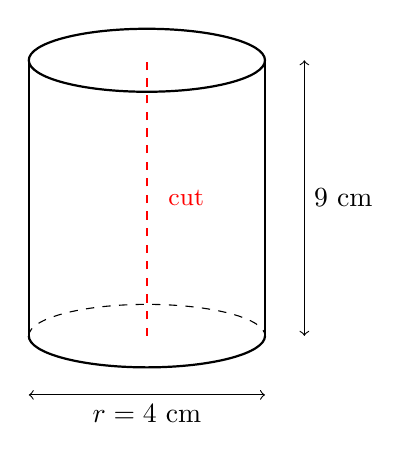
\begin{tikzpicture}[scale=0.5]
  % Cylinder
  \draw[thick] (-3,0) -- (-3,7);
  \draw[thick] (3,0) -- (3,7);
  \draw[thick] (-3,0) arc[start angle=180,end angle=360,x radius=3,y radius=0.8];
  \draw[dashed] (-3,0) arc[start angle=180,end angle=0,x radius=3,y radius=0.8];
  \draw[thick] (-3,7) arc[start angle=180,end angle=360,x radius=3,y radius=0.8];
  \draw[thick] (-3,7) arc[start angle=180,end angle=0,x radius=3,y radius=0.8];
  % Vertical cut line
  \draw[thick,red,dashed] (0,0) -- (0,7);
  \node[right,red] at (0.3,3.5) {\small cut};
  % Labels
  \draw[<->] (-3,-1.5) -- (3,-1.5);
  \node[below] at (0,-1.5) {$r = 4$ cm};
  \draw[<->] (4,0) -- (4,7);
  \node[right] at (4,3.5) {$9$ cm};
\end{tikzpicture}
\end{center}
\end{questionText}
\correctAnswer{Rectangle; $8$ cm by $9$ cm}
\explanation{A vertical cut through the center of a cylinder produces a rectangle. Width = diameter = $2 \times 4 = 8$ cm. Height = $9$ cm.}
\end{practiceQuestion}

\begin{practiceQuestion}{6-8-q10}{mc}
\begin{questionText}
A building is $60$ ft tall and casts a $40$-ft shadow. A nearby tree casts a $12$-ft shadow. How tall is the tree?
\end{questionText}
\choiceA{$8$ ft}
\choiceB{$12$ ft}
\choiceC{$18$ ft}
\choiceD{$20$ ft}
\correctAnswer{C}
\explanation{$\frac{60}{40} = \frac{h}{12}$. Cross-multiply: $40h = 720$. Divide: $h = 18$ ft.}
\end{practiceQuestion}

\begin{practiceQuestion}{7-4-q05}{mc}
\begin{questionText}
A rectangular yard is $20$ m by $15$ m. A circular flower bed with radius $3$ m is in the center. What is the area of the yard NOT covered by the flower bed? Use $\pi \approx 3.14$.
\end{questionText}
\choiceA{$271.74$ m$^2$}
\choiceB{$300$ m$^2$}
\choiceC{$328.26$ m$^2$}
\choiceD{$28.26$ m$^2$}
\correctAnswer{A}
\explanation{Yard: $20 \times 15 = 300$ m$^2$. Circle: $3.14 \times 9 = 28.26$ m$^2$. Remaining: $300 - 28.26 = 271.74$ m$^2$.}
\end{practiceQuestion}

\begin{practiceQuestion}{7-5-q01}{mc}
\begin{questionText}
What is the surface area of a cube with side length $4$ cm?
\end{questionText}
\choiceA{$16$ cm$^2$}
\choiceB{$64$ cm$^2$}
\choiceC{$96$ cm$^2$}
\choiceD{$24$ cm$^2$}
\correctAnswer{C}
\explanation{A cube has $6$ faces. $SA = 6s^2 = 6 \times 16 = 96$ cm$^2$.}
\end{practiceQuestion}

\begin{practiceQuestion}{7-6-q11}{mc}
\begin{questionText}
A triangular prism has a triangular base with legs $5$ cm and $12$ cm (right triangle). The prism is $15$ cm long. What is the volume?
\end{questionText}
\choiceA{$150$ cm$^3$}
\choiceB{$300$ cm$^3$}
\choiceC{$450$ cm$^3$}
\choiceD{$900$ cm$^3$}
\correctAnswer{C}
\explanation{$B = \frac{1}{2} \times 5 \times 12 = 30$ cm$^2$. $V = 30 \times 15 = 450$ cm$^3$.}
\end{practiceQuestion}

\begin{practiceQuestion}{8-1-q23}{sa}
\begin{questionText}
A radio station asks listeners to call in and vote for their favorite song. Explain why this is not a random sample.
\end{questionText}
\correctAnswer{Only listeners who choose to call participate, so it is voluntary and biased}
\explanation{Voluntary response samples are biased because people with strong opinions are more likely to respond.}
\end{practiceQuestion}

\begin{practiceQuestion}{8-2-q28}{gmc}
\begin{questionText}
The table shows how $40$ randomly selected students travel to school.

\begin{center}
\begin{tabular}{|l|c|}
\hline
\textbf{Transportation} & \textbf{Number} \\
\hline
Bus & $16$ \\
\hline
Car & $10$ \\
\hline
Walk & $8$ \\
\hline
Bike & $6$ \\
\hline
\end{tabular}
\end{center}

The school has $600$ students. Predict how many ride the bus.
\end{questionText}
\choiceA{$16$}
\choiceB{$160$}
\choiceC{$200$}
\choiceD{$240$}
\correctAnswer{D}
\explanation{$\frac{16}{40} = 40\%$. Then $40\%$ of $600 = 240$.}
\end{practiceQuestion}

\begin{practiceQuestion}{8-4-q16}{mc}
\begin{questionText}
Group A: $\{60, 65, 70, 75, 80\}$. Group B: $\{40, 55, 70, 85, 100\}$. Both have a mean of $70$. Which group is more variable?
\end{questionText}
\choiceA{Group A}
\choiceB{Group B}
\choiceC{They are equally variable}
\choiceD{Cannot be determined}
\correctAnswer{B}
\explanation{Group A range $= 20$, Group B range $= 60$. Group B's data is far more spread out.}
\end{practiceQuestion}

\begin{practiceQuestion}{8-5-q23}{sa}
\begin{questionText}
The data set is: $28, 31, 33, 36, 40, 42$. What is the median?
\end{questionText}
\correctAnswer{$34.5$}
\explanation{$6$ values: median $= \frac{33+36}{2} = \frac{69}{2} = 34.5$.}
\end{practiceQuestion}

\begin{practiceQuestion}{8-6-q02}{mc}
\begin{questionText}
The full circle in a circle graph represents:
\end{questionText}
\choiceA{$50\%$}
\choiceB{$100\%$ or $360°$}
\choiceC{$180°$}
\choiceD{The largest category}
\correctAnswer{B}
\explanation{The entire circle represents the whole — $100\%$ of the data or $360°$.}
\end{practiceQuestion}

\begin{practiceQuestion}{9-4-q26}{gmc}
\begin{questionText}
Look at the spinner below. Which probability model correctly represents this spinner?

\begin{center}
\begin{tikzpicture}[scale=1.2]
  \fill[funRed!50] (0,0) -- (0:1.5) arc (0:180:1.5) -- cycle;
  \fill[funBlue!50] (0,0) -- (180:1.5) arc (180:270:1.5) -- cycle;
  \fill[funGreen!50] (0,0) -- (270:1.5) arc (270:360:1.5) -- cycle;
  \draw[thick] (0,0) circle (1.5);
  \draw[thick] (0,0) -- (0:1.5);
  \draw[thick] (0,0) -- (180:1.5);
  \draw[thick] (0,0) -- (270:1.5);
  \node at (90:0.8) {\textbf{Red}};
  \node at (225:0.8) {\textbf{Blue}};
  \node at (315:0.8) {\textbf{Green}};
\end{tikzpicture}
\end{center}
\end{questionText}
\choiceA{$P(\text{Red}) = \frac{1}{3}$, $P(\text{Blue}) = \frac{1}{3}$, $P(\text{Green}) = \frac{1}{3}$}
\choiceB{$P(\text{Red}) = \frac{1}{2}$, $P(\text{Blue}) = \frac{1}{4}$, $P(\text{Green}) = \frac{1}{4}$}
\choiceC{$P(\text{Red}) = \frac{1}{4}$, $P(\text{Blue}) = \frac{1}{4}$, $P(\text{Green}) = \frac{1}{2}$}
\choiceD{$P(\text{Red}) = \frac{1}{2}$, $P(\text{Blue}) = \frac{1}{2}$, $P(\text{Green}) = 0$}
\correctAnswer{B}
\explanation{Red covers half the spinner ($180\degree$), while Blue and Green each cover a quarter ($90\degree$ each). This is a non-uniform model.}
\end{practiceQuestion}

\begin{practiceQuestion}{9-6-q15}{mc}
\begin{questionText}
Two dice are rolled. What is the probability that the product (not the sum) of the two numbers is $12$?
\end{questionText}
\choiceA{$\frac{2}{36}$}
\choiceB{$\frac{4}{36}$}
\choiceC{$\frac{3}{36}$}
\choiceD{$\frac{6}{36}$}
\correctAnswer{B}
\explanation{Pairs with product $12$: $(2,6), (6,2), (3,4), (4,3)$ — that is $4$ out of $36$. $P = \frac{4}{36} = \frac{1}{9}$.}
\end{practiceQuestion}

\begin{practiceQuestion}{9-7-q10}{mc}
\begin{questionText}
A student simulates rolling two dice $36$ times to see how often the sum is $7$. They get a sum of $7$ a total of $8$ times. How does this compare to the expected number?
\end{questionText}
\choiceA{Expected: $6$; the simulation result ($8$) is slightly higher}
\choiceB{Expected: $6$; the simulation result ($8$) is much higher}
\choiceC{Expected: $12$; the simulation result ($8$) is lower}
\choiceD{Expected: $7$; the simulation result ($8$) is exact}
\correctAnswer{A}
\explanation{$P(\text{sum} = 7) = \frac{6}{36} = \frac{1}{6}$. Expected: $36 \times \frac{1}{6} = 6$. The simulation gave $8$, slightly above expected.}
\end{practiceQuestion}
